\chapter{The ATLAS Experiment at the LHC}\label{ch3}

The production of massive particles, i.e. top quarks, requires a huge amount of energy. 
Therefore, powerful particle accelerates have been developed for the collision of high energetic initial particles, which allows to use the kinetic energy of those particles for the creation of new heavier objects. Furthermore, complex experimental setups have been constructed to measure the results of those collisions and hence providing data, which is used for the reconstruction of the initial states of interesting events (e.g. $t\bar{t}$ production).

 The dataset used in terms of this analysis has been taken 2015 and 2016 with the ATLAS experiment, in proton-proton collisions, produced by the Large Hadron Collider (LHC), with a center-of-mass energy of 13~TeV. In this chapter the LHC, the ATLAS detector and its subdetector parts will be briefly introduced. Furthermore, a closer description of the trigger and data acquisition system is given as well. 




\section{The Large Hadron Collider}\label{LHC}
\vspace{0.5cm}
\begin{figure}[h]
\centering
\includegraphics[width=1.0\linewidth]{Pics/cp3/31}
\caption{Schematic view of the LHC and its location is given by (a), from reference~\cite{Bruning:2012zz}. The photograph (b) shows a section of the installed LHC in the  tunnel and was made by M. Brice~\cite{Brice:2221112}. }
\label{fig:31}
\end{figure}

 The Large Hadron Collider~\cite{Bruning:2012zz,Bruning:2004ej,Evans:2008zzb} is todays largest and most powerful particle accelerator. It is installed in the underground facilities of the previous Large Electron-Positron Collider (LEP)~\cite{LEP}, which retired after eleven years of operation in the year 2000. The circular tunnel system has a circumference of approximately 27~km and lies between 45 and 170~m below the Swiss-Franco boarder, close to Geneva (see~\cref{fig:31} (a) and (b)). In order to accelerate and collide particles with the same charge, the LHC consists of two beam pipes, which are crossing at four interaction points. In this setup proton-proton ($p-p$), lead-lead ($Pb-Pb$) or proton-lead ($p-Pb$) collisions are performed at the four main LHC experiments: \textbf{ATLAS, CMS, ALICE} and \textbf{LHCb}.

 The two multipurpose detectors ATLAS\footnote{A Toroidal LHC ApparatuS}~\cite{Aad:2008zzm} and CMS\footnote{Compact-Muon-Solenoid}~\cite{Chatrchyan:2008aa} are used for high precision measurements of the Standard Model parameters and the search for new physics. ALICE\footnote{A Large Ion Collider Experiment}~\cite{Aamodt:2008zz} is operating to collect data from heavy ion collisions, for the investigation of the quark-gluon plasma and LHCb\footnote{Large Hadron Collider beauty}~\cite{Alves:2008zz} is built for the search of rare decays and the investigation of CP-violation in the boosted $b\bar{b}$-system. In addition to the four main experiments, placed at the collision points of the LHC, there are the two smaller ones LHCf\footnote{Large Hadron forward}~\cite{Adriani:2008zz} and TOTEM\footnote{Total Elastic and Diffractive Cross Section Measurement}~\cite{Anelli:2008zza}, working on diffractive physics. At last there is the MoEDAL\footnote{Monopole and Exotics Detector at the LHC} experiment~\cite{Pinfold:2009oia}, which focuses on  the search of magnetic monopoles. 
\begin{figure}[h]
	\centering
	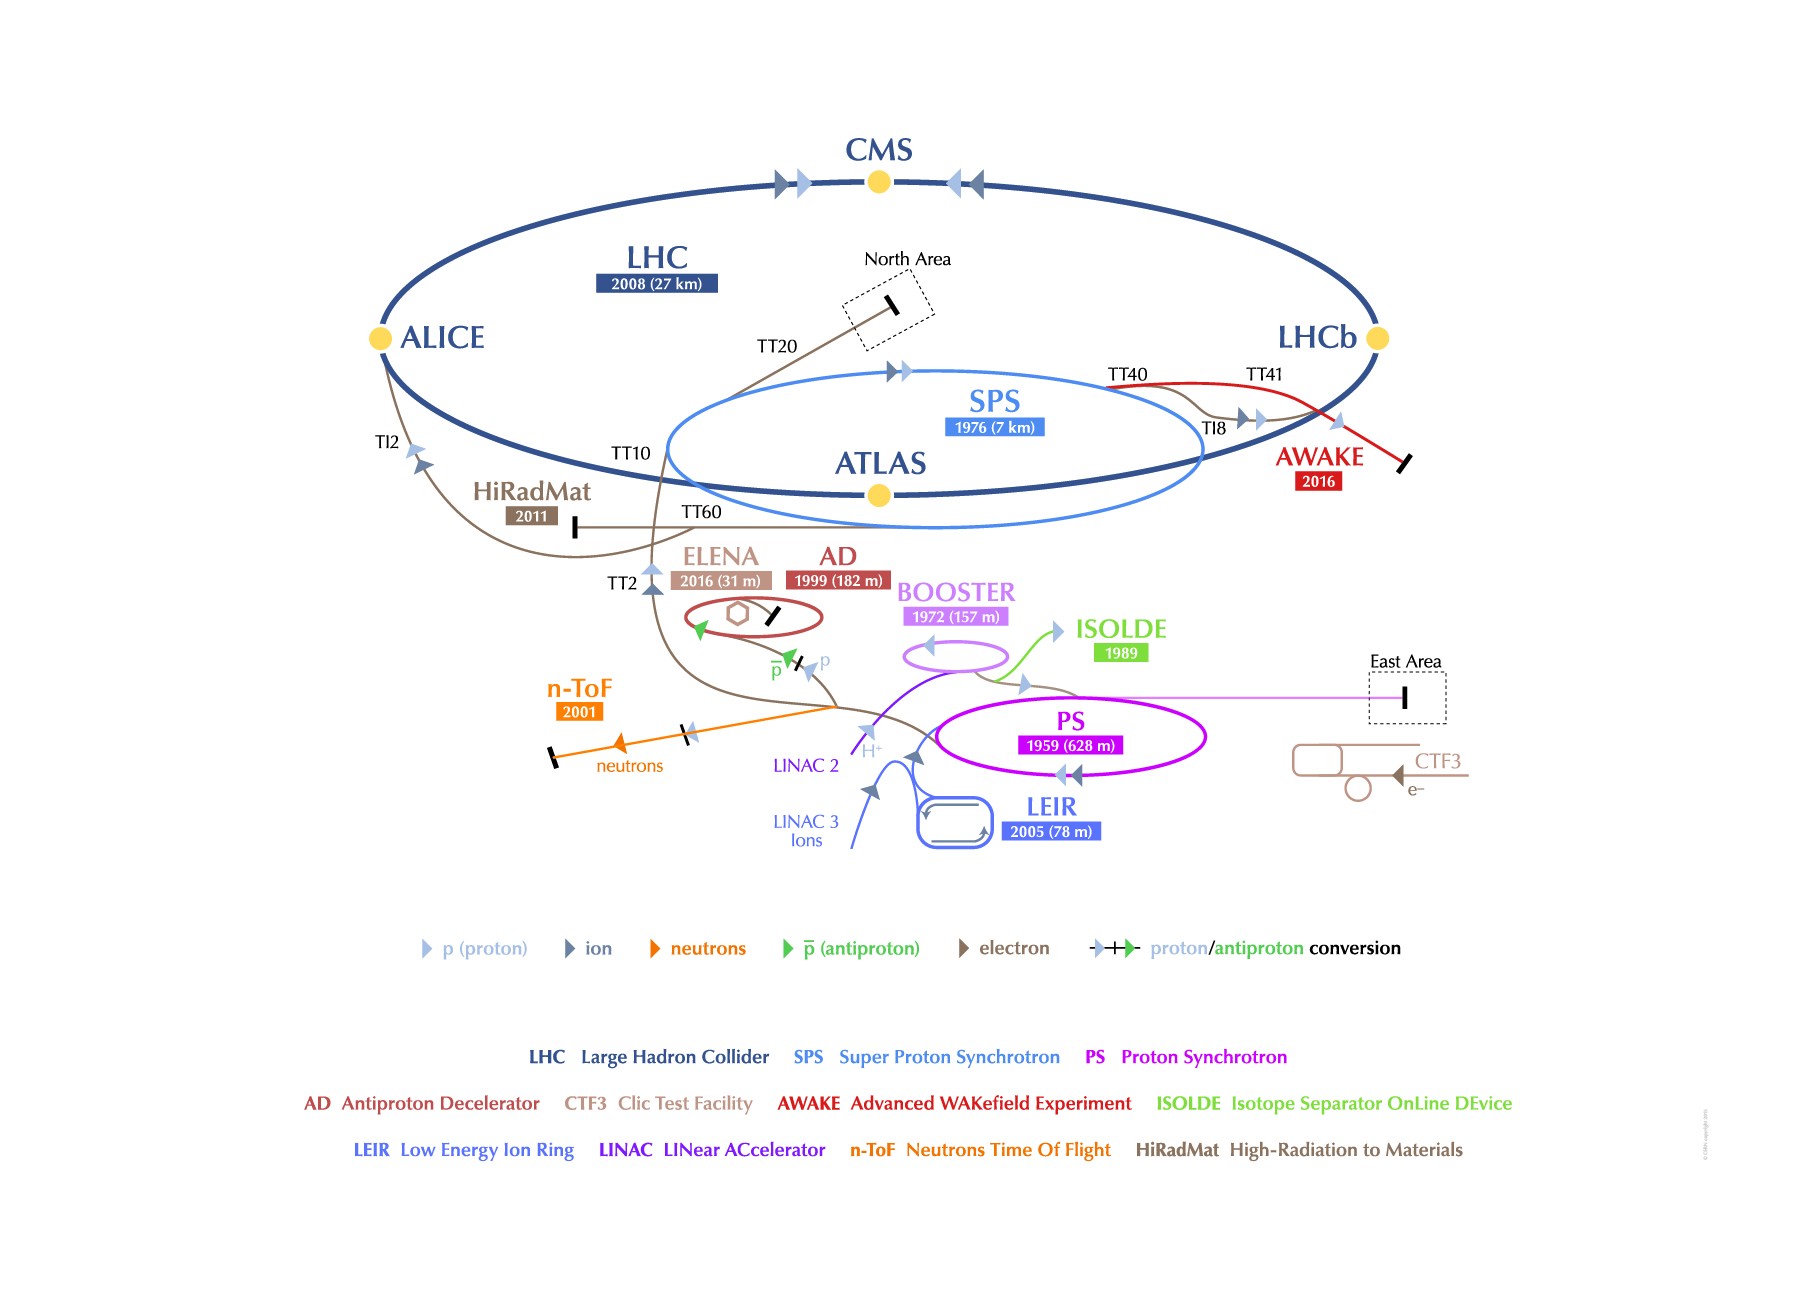
\includegraphics[width=1.0\linewidth]{Pics/cp3/32}
	\caption{Illustration of the whole CERN accelerator complex, with the complete pre-acceleration chain of the LHC~\cite{DeMelis:2119882}.} 
	\label{fig:32}
\end{figure}

 Before the initial particles are brought to collision in the LHC, they first have to pass a chain of pre-accelerators, which is illustrated by~\cref{fig:32}. Protons  are obtained from ionized hydrogen gas and injected in the first accelerator \textbf{LINAC2}, where they are accelerated to an energy of 50~MeV. The next acceleration step is done by the \textbf{Proton Synchrotron Booster (PBS)} that amplifies the proton energies towards 1.4~GeV, followed by the \textbf{Proton Synchrotron (PS)} and the {Super Proton Synchrotron (SPS)}, where the protons reach energies of 25~GeV in the first one and finally 450~GeV in the later one. After the SPS, the particles are injected into the {LHC}, where the acceleration continuous up to the peak energy of currently 6.5~TeV.

 These accelerated protons, in each beam-pipe of the LHC, are grouped into bunches of 10$^{11}$ particles with a bunch spacing of 25~ns. This bunches are accelerated in the LHC by sixteen superconducting radio-frequency cavities. 1232 main superconducting dipole and 392 main superconducting quadruple magnets are used for the guiding and the focusing of the particle beams along the beam-pipe. These magnets are cooled by superfluid helium below 2~K and a have a maximal field strength above 8~TeV~\cite{Evans:2008zzb}.   


 The LHC  exceeds all experiences in terms of luminosity with previous hadron colliers. The peak luminosity is defined by:
\begin{equation}
\mathscr{L} = \frac{\gamma N_1N_2n_1n_2f}{4\pi \sigma_x \sigma_y }.
\end{equation}
 It depends on the number of particles $N_i$ in each bunch, as well as of the total number of bunches $n_i$ in the LHC, the revolution frequency $f$ and the cross-sections $\sigma_i$ of the incoming particle bunches. $\gamma$ denotes the relativistic coefficient. Design goal for the LHC has been to achieve a peak luminosity of O($10^{34}$~1/cm$^2$s$^{-1}$), at a center-of-mass energy of 14~TeV~\cite{Bruning:2004ej}. For 2015/2016 at 13~TeV the peak luminosity was 1.38$\cdot$10$^{34}$~1/cm$^2$s$^{-1}$.  
 
 
\section{The ATLAS Experiment}\label{ATLAS}
 ATLAS  is one of the two multipurpose detectors at the LHC and has obtained the dataset used in this analysis. It measures 44~m in length and 25~m in diameter and weighs around 7000~t~\cite{Aad:2008zzm}. 
 As shown by~\cref{fig:33}, it covers almost a full 4$\pi$ solid angle and has a forward-backward symmetry, which is realized by the so-called barrel around the collision center and the two end-caps. The detector is built up with an onion-shell structure, consisting of various sub-detector layers. The three main subcomponents of the ATLAS detector are:
 \begin{itemize}
 	\item the \textbf{Inner Detector system (ID)}, for the reconstruction of particle trajectories, 
 	\item  the \textbf{Calorimeter System (CS)}, which is measuring particle energies
 	\item  and the \textbf{Muon Spectrometer (MS)}, for the determination of the muon momentum.
 \end{itemize} 
Characteristic for the ATLAS experiment is the huge superconducting air-core toroid system, which is used for the deflection of muons in the MS. 

 The different detector components are optimized in order to identify and distinguish between the different constituents of a collision, facing difficulties like high particle multiplicities and high event rates. Therefore,  additionally  efficient triggering and fast read-out electronics is required, to distinguish between background and signal.

The different layers of the ATLAS experiment will be briefly discussed after a short introduction of the detector coordinate system. For a more detailed information, the reader is refereed to~\cite{Aad:2008zzm,ATLAS:1999uwa}.   


\begin{figure}[t]
	\centering
	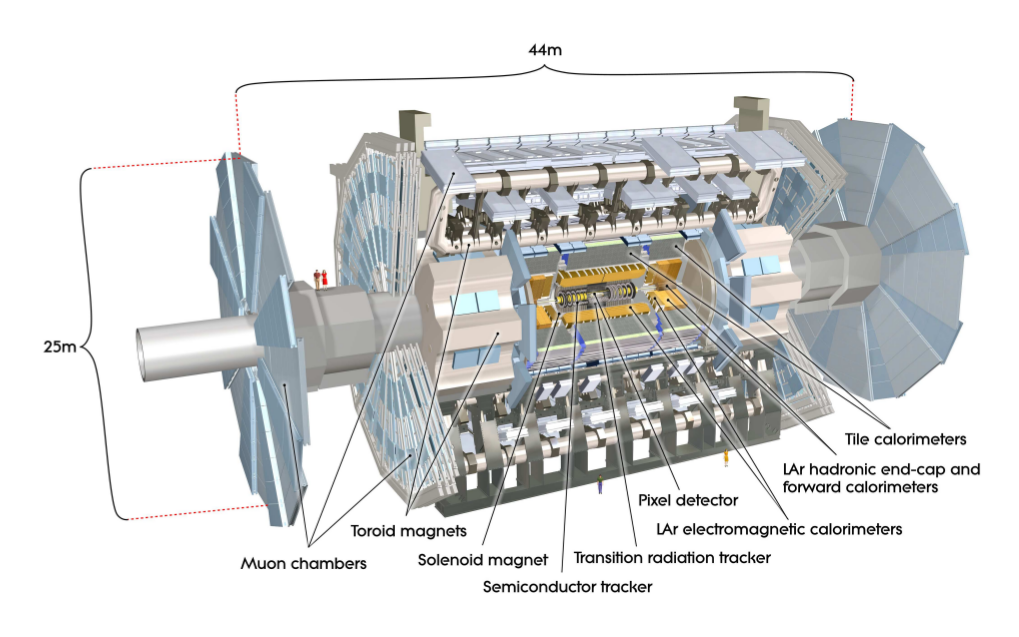
\includegraphics[width=1.0\linewidth]{Pics/cp3/33}
	\caption{The ATLAS experiment and its sub-structure~\cite{Aad:2008zzm}.} 
	\label{fig:33}
\end{figure}



\subsubsection{The Coordinate System}\label{Coordinate}
The cylindrical shape of the ATLAS experiment implies the use of a polar coordinate system, with the z-axis  parallel to the beam-pipe and the particle collision point in the origin of the coordinate system. The x-axis is defined to point inwards to the LHC center, while the y-axis lies perpendicular to the x-z plane, pointing upwards. For the polar angle $\Theta$ and the azimuthal angle $\phi$, the standard definition are used. Furthermore, the cylindrical coordinate system can be adopted, using the polar angle, by the so-called pseudorapidity
\begin{equation}\label{pseudorapidity}\eta = -\text{ln}\left(\text{tan}\left(\frac{\Theta}{2}\right)\right).
\end{equation}  
 For the interesting central detector area, close to the y-axis,  $\mid\eta\mid$ takes low values and offers a high resolution, while in the background dominated section $\mid\eta\mid$ increases rapidly with declining distance to the beam pipe. Thus, this high $\mid\eta\mid$  region is often excluded in the measurements. In addition, the introduction of the pseudorapidity provides with $\Delta \eta$ - the distance between to distinguishable values- a quantity which is invariant under Lorentz transformations along the z-axis. Furthermore, for massless objects, the pseudorapidity is equal to the so-called rapidity, which is defined as:
\begin{equation}\label{rapidity}
y = \frac{1}{2}\text{ln}\left(\frac{E + p_z}{E - p_z}\right).
\end{equation}
$E$ denotes the total energy and $p_z$ the third component of the particles momentum. The rapidity is invariant under Lorentz transformations and used for the description of very massive objects, i.e.  jets.


The distance of two different particles $i$ and $j$ is described by:
\begin{equation}\label{dinstance}
\Delta R_{i,j} = \sqrt{(\eta_i-\eta_j)^2+(\Theta_i-\Theta_j)^2}.
\end{equation}
   

The hadron sub-structure gives rise to further issues. The momentum fraction $x$ carried by the different partons can not determined exactly, because the PDFs allow only to take the probability, that a parton has a certain $x$, into account. Therefore, the absolute values of the parton momenta and energy are unknown. Nevertheless, the transfer components $E_T$,$p_x$ and $p_z$, of the initial partons sum up to zero. This is also assumed for the final state partons with their transfer components:
 \begin{equation}
 p_T = \sqrt{p_x^2+p_y^2} \text{\hspace{0.3cm} and \hspace{0.3cm}} E_T =E \cdot \text{sin}(\Theta).
 \end{equation}        





\subsection{The Inner Detector System}\label{ID}
The Inner Detector System (ID) of the ATLAS experiment, is designed to reconstruct the tracks, as well as the primary and secondary vertices, by the interaction of the charged particles with the detector material. Therefore, the ID consist of three sub-components, which are designed to provide a high vertex and momentum resolution, due to  very fine granular structures.

The whole ID system is composed out of a cylindrical part, located in the barrel around the collision point, and the corresponding detector end-caps. It measures around 7~m in length and has a diameter of 2.3~m. The complete ID is contained in a solenoidal magnetic field of 2~T, which is used for bending charged objects and resolving the sign of the charges. The required precise resolution is realized by the use of discrete space-points from several silicon pixel layers at the most inner region of the ID (see~\cref{fig:34}).

 The \textbf{Silicon Pixel Detector}, closest to the collision center, is built out of three layers parallel and three disks perpendicular to the beam pipe, with 1744 sensor modules in total. It is mainly used together with \textbf{Semiconductor Tracker (SCT)}, which is installed in the layers above, for the momentum measurement and the vertex reconstruction. The SCT consists out of four silicon strip layers in the barrel and in total eighteen disks for both end-caps. This results in a total number of 3100 modules. The 12~cm silicon strips are composed out of two connected sensors, often refereed as dual layer design. The sensors are connected with readout electronics.

 At the outer radii of the ID, the \textbf{Transition Radiation Tracker (TRT)} is placed.
It uses the information arising from the transition radiation of passing particles, to distinguish e.g. between electrons and pions. The TRT is built out of several layers of straw tubes filled with a gas mixture of XeCO$_2$ and O$_2$. While the TRT is constructed to operate at room temperature, the silicon sensors of the detector have to be cooled down between -5 and -10~\textdegree C, to get a satisfactory noise performance and long term reliability, while suffering under the high radiation close to the beam-pipe~\cite{Aad:2008zzm}.     
\begin{figure}[t]
	\centering
	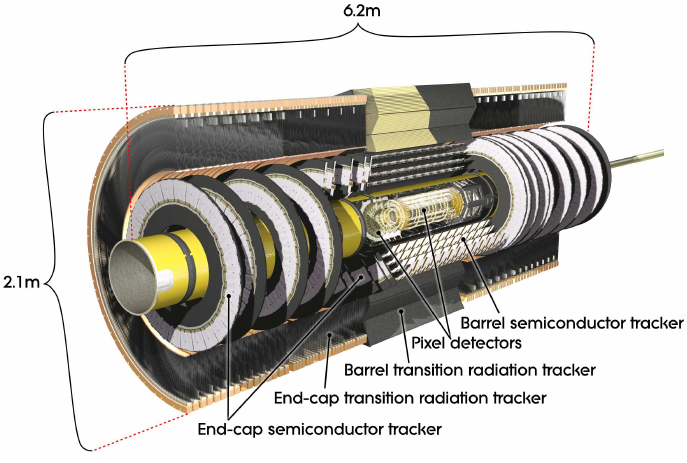
\includegraphics[width=0.7\linewidth]{Pics/cp3/34}
	\caption{Cut through the Inner Detector System~\cite{Aad:2008zzm}.} 
	\label{fig:34}
\end{figure}

\subsection{The Calorimeter System}\label{CD}




The second detector shell is specifically developed for the measurement of energies induced by particle showers, also known as clusters. 
Electrons, positrons and photons deposit most of their energy in the inner layer, which is called the \textbf{Electromagnetic Calorimeter (EC)}.  The particles interact with the  detector marital, e.g. via electron-positron pair production and annihilation or the radiation of bremsstrahlung. Thus, secondary particles are triggered by the passing ones, resulting in electromagnetic showers. If the incident particles are hadrons, the same phenomena occurs, due to inelastic scattering  of the hadrons with the nuclei of the detector material. The scattering processes lead to the production of new hadrons, which participate in further interactions and therefore creating a hadronic particle shower, which is also detected by the EC and in addition by the outer \textbf{Hadronic Calorimeter (HC)}. Despite the energy measurement, the Calorimeter System also allows to determine the  particle momentum and identity, by the analysis of direction and spatial characteristics of the clusters.

The Calorimeter System has a  cylindrical shape, which measures 12.20~m in length with radius of 4.25~m (see~\cref{fig:35}). It is built out of so-called sampling detectors, which are alternating structures of layers with a passive and an active component.

 The passive material interacts with the incident particles and triggers the particle shower, while the active material gets ionized by the passing particles from the shower and provides information for the electronic read out. In case of the ATLAS Calorimeter System, liquid argon (LAr) is the preferred choice for the active part, because of the intrinsic linear response and the excellent radiation hardness~\cite{Aad:2008zzm}. A cryogenic system is used for a constant operational temperature of 87~K.


\begin{figure}[h]
	\centering
	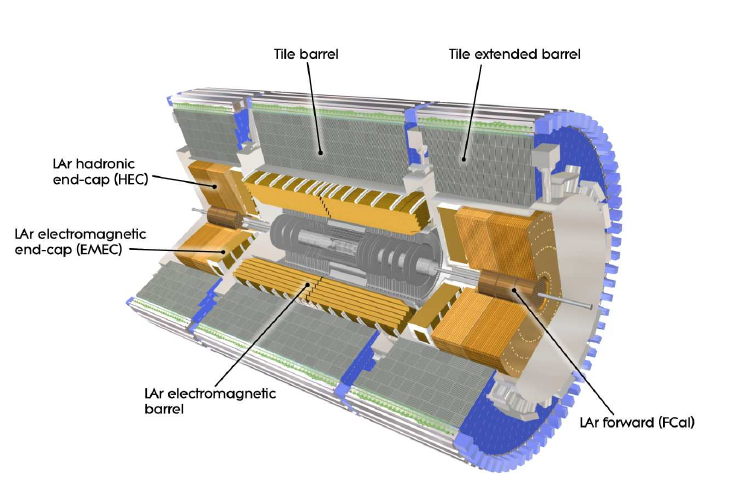
\includegraphics[width=0.65\linewidth]{Pics/cp3/35}
	\caption{Cut through the Calorimeter  System~\cite{Aad:2008zzm}.} 
	\label{fig:35}
	\end{figure}



 The \textbf{Electromagnetic Calorimeter} is built out of two units with a length of 3.2~m in the barrel region, plus two end-cap wheels. Lead is used for the passive and liquid argon for the active media. The kopton electrode layers have a characteristic accordion shape, which allows to cover a decent $\Phi$  and $\mid\eta\mid$ range, e.g. the area for high precision measurements  ($0 \leq~  \mid\eta\mid ~\leq 2.5$) is covered, as well as the high-$\eta$ area  ($2.5 \leq~ \mid\eta\mid~ \leq3.2$). In front of the EC, a presampling layer is installed, to measure energy losses  from particle interactions with the ID, the superstructure and the beam pipe.




For the detection of particle showers from quarks and gluons the \textbf{Hadronic Calorimater} is installed and enveloping the EC. While both calorimeters are used for the observation of hadron jets, the most amount of energy is deposited in the latter one, which uses scintillator tiles and steel absorbers in the inner region. In this so called \textbf{Tile Calorimeter (TC)}, the scintillators act as active media, which creates photons by the interaction with the incident particles. Wavelength shifters and photomultipliers are  used for the generation and amplification of the electrical signal. The TC has a inner radius of 2.28~m and a outer one of 4.25~m. It is built out of a central barrel with a length of 5.8~m, plus two extended barrels, measuring 2.6~m in length. This construction  allows to cover a pseudorapidity range of $0 \leq \mid\eta\mid \leq1.7$.

 Larger $\eta$ regions are taken into account by the \textbf{Hadronic End-Cap Calorimeter (HEC)} and the \textbf{Forward Calorimeter (FCal)}, which enable to observe a pseudrapidity range up to 4.9.  In the HEC, copper and liquid argon are used as sampling media. In each of the end-caps, two cylindrical HEC wheels with a radius of 2.03~m are embedded, resulting in the coverage of the section: $1.5 \leq \mid\eta\mid \leq3.2$.

 The FCal is placed in the same segment as the HEC, covering the $3.1 \leq \mid\eta\mid \leq 4.9$. It uses copper and tungsten for the passive sampler, combined with liquid argon for the active one. The mixture of the two passive media is a choice, in consequence of the high particle flux in the operating $\eta$ region of the FCal, which stresses the detector material quit extensively.




\subsection{The Muon Spectrometer}\label{MD}

\begin{figure}[h]
	\centering
	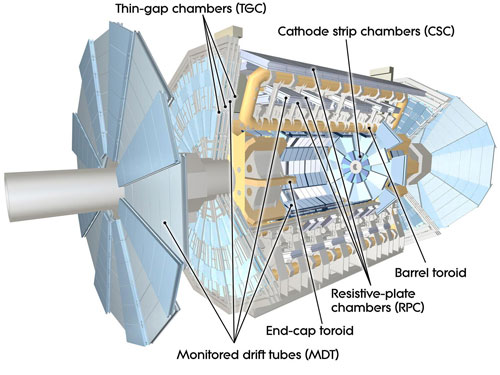
\includegraphics[width=0.65\linewidth]{Pics/cp3/36}
	\caption{The Muon Spectrometer with all its sub-components~\cite{Aad:2008zzm}.} 
	\label{fig:36}
\end{figure}

 The momenta of muons leaving the calorimeter are measured in the outer most layer of the ATLAS experiment, the \textbf{Muon Spectrometer (MS)}. Together with the informations provided from the Inner Detector System, the measurements of the MS can be used for the reconstruction of the muon trajectories. Furthermore, the MS works also as a trigger for events with muons.

The track reconstruction in the MS is based on the magnetic deflection of the muons, by a large superconducting air-core toroid magnet system in combination with a trigger and several kinds of tracking chambers. The design goal of the whole Muon Spectrometer is to achieve a momentum resolution of 10~\% for 1~TeV and up to 3~\% for 10-200~GeV muons~\cite{ATLAS:1999uwa}. The instrumentation design was mainly dictated by the high particle flux, which has huge impacts on the operational performance, considering e.g. aging and agglomeration of polymers, high rate capability and radiation hardness.

 The complete system (see~\cref{fig:36}) consist of three barrel layers with radii of  5~m, 7.5~m and 10~m, as well as of four end-cap wheels, located at $\mid z \mid$ = 7.4~m, 10.8~m, 14~m and 21.5~m. 
With increasing radii also the dimensions of the different layers and their components ,i.e. the chambers, gain in size. In the barrel, as well as in the end-cap region, \textbf{Monitoral Drift Tubes (MDT)} and \textbf{Cathode Strip Chambers (CSC)} provide high spatial resolution, due to the fact, that the systems are monitored with an optical alignment system, which provides excellent spatial informations. Moreover, \textbf{Resistive Plate Chamber (RPC)} in the barrel and \textbf{Thin Gap Chambers (TGC)} in the forward section are  installed for additional trigger information.



 For the magnetic bending of the muons, a unique superconducting \textbf{Magnetic System} is installed in the MS. Together with the solenoid of the ID, it allows, the determination of the sign of the particles charge, as well as a high-precision measurement of the particle momentum. The MS system is composed of one large barrel toroid and two smaller toroids in the end-caps (see~\cref{fig:37}). It measures about 26~m in length, with a diameter of 22~m and provides a specific magnetic field configuration, resulting in orthogonal alignment of the field towards the muon trajectory~\cite{ATLAS:1999uwa}. In the transition region, between barrel and end-caps, the magnetic field is reduced, while in general it is  non-uniform distributed  with a field strength of 4.7~T.  A cryogenic system with liquid helium is used to cool down the system to 1.8~K. Furthermore,  each coil has an air core, for the noise reduction due to  multiple scattering processes of the muons. 

\begin{figure}[h]
	\centering
	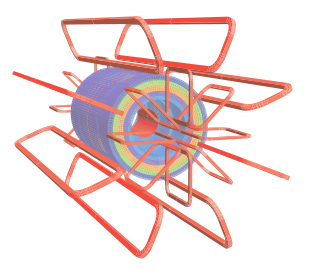
\includegraphics[width=0.4\linewidth]{Pics/cp3/37}
	\caption{Illustration of the ATLAS Magnet System, with the inner solenoid of ID and the large superconducting coils of the MS ~\cite{Aad:2008zzm}.} 
	\label{fig:37}
\end{figure}



 The \textbf{Monitorial Drift Tube} System consists of rectangular  chambers, which measure between 1~m and 6~m in length and 1~m up to 2~m in with. The chambers contain several layers of cylindrical drift tubes, filled with a gas mixture of Ar(30~\%) and CO$_2$ (70~\%) at a nominal  pressure of 3~bar. Incident muons, ionize the the argon gas and create free electrons, which drift towards the central tungsten-rhenium anode wire of the tube, producing an electron avalanche.  The anode has a diameter of 50~$\mu$m and a potential of 3080~V. The end-plugs are designed to hold the wire in position with an accuracy smaller than 10~$\mu$m and are connected to the read out electronics. The CO$_2$ is used as quench gas, to eliminate additional interaction processes, which could for example arise from electrons ripped out of the cathode. 

 The use of MDTs is limited by the counting rates (150~Hz/cm$^2$), which are exceeded in the forward region. Therefore, MDTs are replaced by \textbf{Cathode Strip Chambers}, which are able to handle the high particle flux in the end-cap region by providing counting rates up to 1000~Hz/cm$^2$~\cite{ATLAS:1999uwa}. There are two disks in the detector wheels, each containing 8 CDCs. The CDCs are multi-wire proportional chambers, with cathode stripe  and anode wires orientated in radial direction. The chambers are filled with a gas mixture of  80~\% Ar and 20~\% CO$_2$, acting as quench gas. The track reconstruction is based on the information of induced charge in the anode wires, created by the ionized argon.

 For the particle triggering, three trigger layers of \textbf{Resistive Plate Chambers (RPC)}, are embedded  in between the MDTs. Each of this so-called trigger stations consist of two separate sub-layers. Thus a particle passing trough provides multiple informations, which help to reduce noise.  The RPCs are parallel-plate detectors, where electron avalanches are formed by an electrical field (49~kV/m) between two electrodes, which are separated by about 2~mm by an insulating material. The RPCs are filled with a gas mixture of 94.7~\%   C$_2$H$_2$F$_4$, 5~\% Iso-C$_4$H$_{10}$ and 0.3~\% SF$_6$, which allows for example to work with  low voltages~\cite{ATLAS:1999uwa}. 

Additional trigger information in the end-cap regions is obtained by \textbf{Thin Gap Chambers (TGCs)}. These are multi-wire proportional counters, where the anode wires 
measure the radial coordinate of the particle track and outer strip electrodes provide the azimuthal information. The ATLAS TGCs are operating a gas combination of CO$_2$ and n-C$_5$H$_{12}$, which offer high quench capabilities.


\section{Trigger System and Data Acquisition}


 The amount of information produced due to the  high luminosity and large bunch-crossing rate of 40~Mhz at the LHC, makes it impossible to store all the data. Furthermore, only a fraction of all interactions result in interesting events, e.g. $t\bar{t}$ production. Therefore, the ATLAS collaboration works with a \textbf{three level trigger system}. That so-called trigger stations consist of a hardware-based Level 1 trigger (L1), the software based Level 2 trigger (L2) and the Event Filter (EF). For the second run period of the LHC (Run 2), the L2 trigger and the Event Filter are merged in  the~\text{High Level Trigger} (HLT). In order to reduce to the complexity of the system the following explanation will stick to the three levels of the trigger system. The complete trigger system is illustrated in~\cref{fig:38} 

The amount of raw data, which passes the trigger system is still impressive. For storage, as well as for further analysis the \textbf{Worldwide LHC Computing Grid} is used.

\begin{figure}[t]
	\centering
	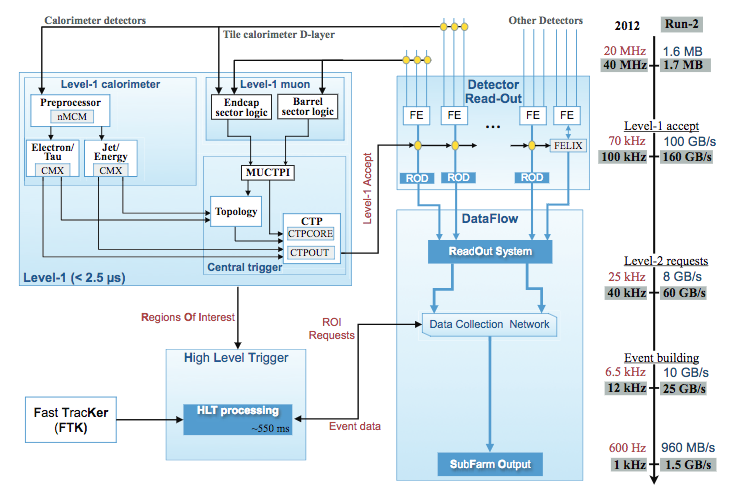
\includegraphics[width=0.80\linewidth]{trigger}
	\caption{Sketch of the three level trigger system~\cite{Nakahama:2015211}.} 
	\label{fig:38}
\end{figure}


 The entirely hardware based \textbf{L1} trigger station uses for its selection, information from the Calorimeter System and from the Muon Spectrometer. L1 searches for high $p_T$ muon, electrons, jets and missing transverse energy. This data is used for the definition of Regions of Interests (RoI), which will be used for the further refinement and selection by the next trigger stations. Therefore, the events are stored in so-called Read-Out-Drivers (ROD). It takes about 2.5~$\mu$s, for the complete selection of the RoIs, which leads to a reduction of the event rate towards 100~kHz. The second trigger station \textbf{L2} is software-based and takes the complete detector information of the RoIs into account. For the selection of this trigger station large computational facilities are used. The event rate after L2 is reduced to about 12~kHz. 
Events that survive this selection step, are passed to the Event Filter.

 The final step of the trigger process is the \textbf{EF}, there a full reconstruction of the different constituents of the event, with all available information, is performed. The physical objects and their properties, e.g.  tracks and vertices are rebuilt. At last the selected events are saved permanently. The final event rate after the EF is 1~kHz and the data rate is 1.5~GB/s~\cite{Nakahama:2015211}.






\subsection{Data Handling}

 In order to handle the storage of the huge amount of data, as well as providing the necessary computational infrastructure, e.g. for Monte Carlo simulations, the\textbf{ Worldwide LHC Computing Grid (WLCG)} has been developed. Its based on large computational facilities around the globe, which are shearing their storage capabilities and processing power. This computer network is structured into different hierarchies, where the CERN computing center has the highest, so-called  Tier-0,  rank. There are stored copies of all raw data sets. Furthermore, there are backups at eleven computer centres around the globe, which are the so-called Tier-1 centers. Moreover,  the smaller Tier-2 centers are used to store copies of selected data and to provide the necessary resources for the data analysis and the simulation of events via Monte Carlo generators. The datasets are stored in streams and reconstructed within 24h.


\subsection{Detector Simulation}
This analysis uses the template method, which is based on simulated Monte Carlo distributions. In order to compare the simulated events to measured data, a detailed simulation of the ATLAS detector has been developed. 
The detector simulation is based on the \text{Geant4}~\cite{Agostinelli:2002hh} program  and starts from the event generation. The provided output of the simulation has a format, which can be compared to the data measured with the real detector.  
 A description of the detector simulation is given by~\cite{Aad:2010ah}. 
 
 The first step is the event generation, where a set of particles is produced and passed through the detector simulation. 
For the event generation, several standard physics generators can be used. 
 The generated events consist of particles  related to a single interaction, where the corresponding vertex is located at the geometric origin. 
 Particles which have a decent lifetime (30~ps) are treated as stable particles. These particles are considered to be able to interact with the detector material and their decay is taken into account by the simulation. For short living particles, the decays are handled by the event generator itself. The corresponding interactions with the detector material are ignored.  
The core simulation within  \text{Geant4} models the particle transportation through the detector geometry and takes additional information provided by the user into account. The hits,  produced by the simulation, are converted into detector responses. These so called digits are produced  if the corresponding electrical signal in the readout-channels exceeds a defined threshold in certain time range. ~\cite{Aad:2010ah} 

After the detector simulation, the simulation data is passed through the same event reconstruction software as the data.
A correct simulation of the detector is generally  important for the physics analysis. Deviations in the simulation can  for example be observed by comparing the data to the simulation.
